\documentclass[oneside,14pt]{extarticle}
\usepackage[utf8]{inputenc}
\usepackage[english,ukrainian]{babel}
\usepackage{amssymb,amsfonts,amsmath,amsthm,mathtext,textcomp}

\usepackage[includehead, headsep=0pt, footskip=0pt, top=2cm, bottom=2cm, left=2cm, right=1cm]{geometry}
\usepackage{indentfirst}
\usepackage[onehalfspacing]{setspace}
\usepackage[headings]{fancyhdr}
\usepackage{etoolbox}
\usepackage{flafter}
\usepackage{listings}
\usepackage{graphicx}
\usepackage{float}
\usepackage[labelsep=period]{caption}
\lstset{
	breaklines=false
}
\usepackage{array}
\fancyhf{}
\renewcommand{\headrulewidth}{0pt}
\pagestyle{fancy}
\fancyfoot[R]{\thepage}
\lstset{breaklines=true,}
\graphicspath{ {./pictures} }

\lstset{
	language=c,
	tabsize=4,
	keepspaces,
	showstringspaces=false,
}
\graphicspath{ {./pictures} }
\setlength{\parindent}{4em}
\setlength\tabcolsep{5px}

\newcommand\subject{Моделювання та аналіз програмного забезпечення}
\newcommand\lecturer{доцент кафедри ПЗ \\ Сердюк П.В.}
\newcommand\teacher{викладач кафедри ПЗ \\ Микуляк А.В.}
\newcommand\mygroup{ПЗ-22}
\newcommand\lab{4}
\newcommand\theme{Структурні шаблони проектування}
\newcommand\purpose{Здобути навички використання структурних шаблонів проектування при моделюванні програмних систем}

\begin{document}
\begin{normalsize}
	\begin{titlepage}
		\thispagestyle{empty}
		\begin{center}
			\textbf{МІНІСТЕРСТВО ОСВІТИ І НАУКИ УКРАЇНИ\\
				НАЦІОНАЛЬНИЙ УНІВЕРСИТЕТ "ЛЬВІВСЬКА ПОЛІТЕХНІКА"}
		\end{center}
		\begin{flushright}
			\textbf{ІКНІ}\\
			Кафедра \textbf{ПЗ}
		\end{flushright}
		\vspace{70pt}
		\begin{center}
			\textbf{ЗВІТ}\\
			\vspace{10pt}
			до лабораторної роботи № \lab\\
			\textbf{на тему}: “\textit{\theme}”\\
			\textbf{з дисципліни}: “\subject”
		\end{center}
		\vspace{50pt}
		\begin{flushright}
			
			\textbf{Лектор}:\\
			\lecturer\\
			\vspace{10pt}
			\textbf{Виконав}:\\
			
			студент групи \mygroup\\
			Коваленко Д.М.\\
			\vspace{10pt}
			\textbf{Прийняв}:\\
			
			\teacher\\
			
			\vspace{28pt}
			«\rule{1cm}{0.15mm}» \rule{1.5cm}{0.15mm} 2023 р.\\
			$\sum$ = \rule{1cm}{0.15mm}……………\\
			
		\end{flushright}
		\vspace{\fill}
		\begin{center}
			\textbf{Львів — 2023}
		\end{center}
	\end{titlepage}
		
	\begin{description}
		\item[Тема.] \theme.
		\item[Мета.] \purpose.
	\end{description}

	\section*{Завдання}
Розробити структурні шаблони проектування відповідно до прецедентів обраного
варіанту ігрової логіки. Вибрати один з прецедентів, для якого найбільш доцільно
застосувати структурний шаблон (не всі прецеденти цього потребуватимуть).

	Представити діаграму класів ігрового проекту (із відображенням на ній використаних
	шаблонів).

	\section*{Хід виконання}
	
	\begin{figure}[H]
		\centering
		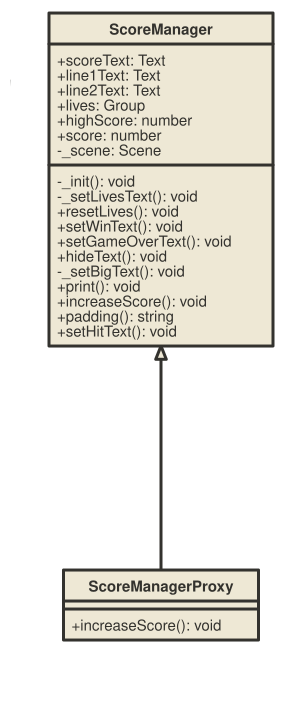
\includegraphics[]{proxy}
		\caption{UML діаграма реалізації шаблону Proxy}
	\end{figure}
	
	\begin{figure}[H]
		\centering
		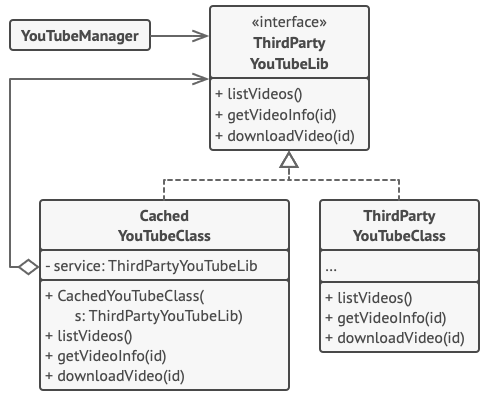
\includegraphics[]{proxy-ex}
		\caption{UML діаграма прикладу реалізації шаблону Proxy}
	\end{figure}
	
	\begin{small}
		\begin{lstlisting}
export class ScoreManagerProxy extends ScoreManager {
	constructor(_scene: Phaser.Scene) {
		super(_scene);
	}
	
	increaseScore(step = 10) {
		super.setHitText();
		super.increaseScore(step);
	}
}
		\end{lstlisting}
	\end{small}
	
	\begin{figure}[H]
		\centering
		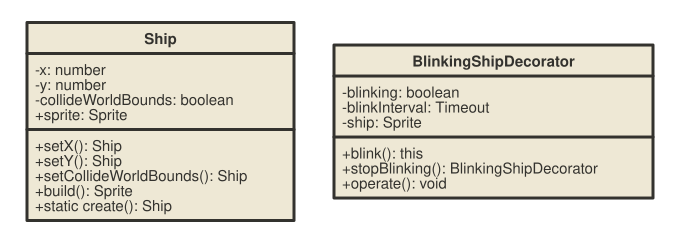
\includegraphics[width=\textwidth]{decorator}
		\caption{UML діаграма реалізації шаблону Decorator}
	\end{figure}
	
		\begin{figure}[H]
		\centering
		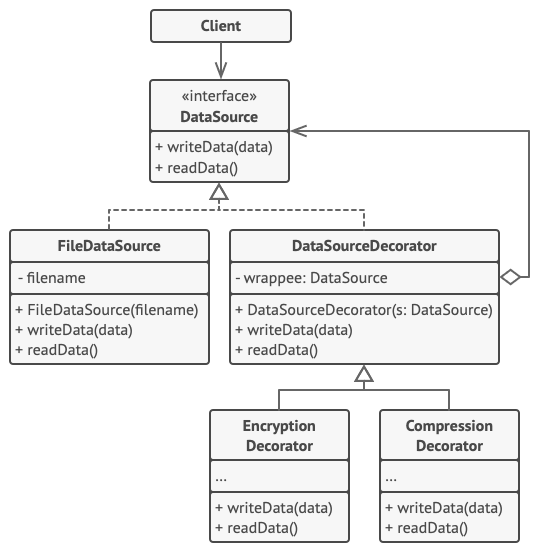
\includegraphics[width=\textwidth]{decorator-ex}
		\caption{UML діаграма прикладу реалізації шаблону Decorator}
	\end{figure}
	
	\begin{small}
		\begin{lstlisting}
			
			export class BlinkingShipDecorator {
				private blinking: boolean = false;
				private blinkInterval: NodeJS.Timeout | null = null;
				private ship: Phaser.Physics.Arcade.Sprite;
				
				constructor(ship: Phaser.Physics.Arcade.Sprite) {
					this.blinking = false;
					this.ship = ship;
				}
				
				blink(interval: number = 200) {
					if (!this.blinking) {
						this.blinking = true;
						this.blinkInterval = setInterval(() => {
							if (this.ship) {
								this.ship.setVisible(!this.ship.visible);
							}
						}, interval);
					}
					
					return this;
				}
				
				stopBlinking(): BlinkingShipDecorator {
					if (this.blinking) {
						if (this.blinkInterval) {
							clearInterval(this.blinkInterval);
						}
						this.ship.setVisible(true);
						this.blinking = false;
						this.blinkInterval = null;
					}
					
					return this;
				}
				
				operate() {
					console.log("operate");
				}
			}
			
		\end{lstlisting}
	\end{small}
	
	\begin{figure}[H]
		\centering
		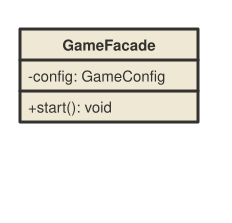
\includegraphics{facade}
		\caption{UML діаграма реалізації шаблону Facade}
	\end{figure}
	
		\begin{figure}[H]
		\centering
		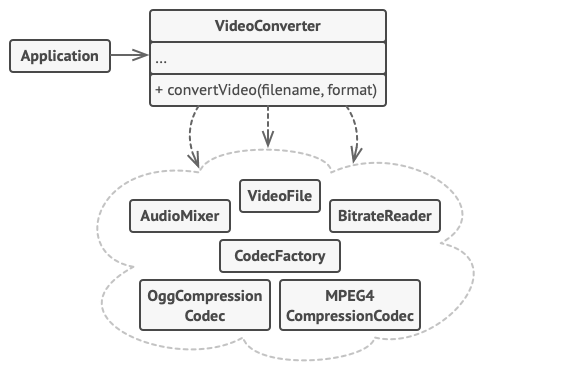
\includegraphics{facade-ex}
		\caption{UML діаграма прикладу реалізації шаблону Facade}
	\end{figure}
	
	\begin{small}
		\begin{lstlisting}
import "phaser";
import { MainScene } from "./scenes/main";

class GameFacade {
	private config: Phaser.Types.Core.GameConfig;
	
	constructor() {
		this.config = {
			title: "lab",
			type: Phaser.AUTO,
			backgroundColor: "rgb(47, 52, 55)",
			width: 800,
			height: 600,
			scene: MainScene,
			physics: {
				default: "arcade",
			},
			parent: "Lab",
		};
	}
	
	start() {
		new Phaser.Game(this.config);
	}
}

const gameFacade = new GameFacade();
gameFacade.start();

		\end{lstlisting}
	\end{small}
	
	\section*{Висновки}
	   Під час виконання лабораторної роботи я здобув навички використання структурних шаблонів проектування при моделюванні програмних систем.
\end{normalsize}
\end{document}
